% -*- TeX -*- -*- UK -*- -*- Soft -*-"

\chapter{Setting DVIPS}

\section{DVIPS settings}

If you are using DVIPS: do the following.


\subsection{Enable Colour PNG in DVIPS}

DVIPS converts \TeX{} DVI files into PostScript files.

DVIPS only supports EPS files as input graphics. If you use DVIPS and you want to use PNG files, you need to use bmeps to convert the PNG to an EPS first. Fortunately bmeps is included in the MikTex DVIPS (a so-called 'bmeps enabled DVIPS' version).  Unfortunately the default WinEdt mode only converts the files to a monochrome EPS file, destroying all colour information.  The switch to convert PNG files to EPS format in colour must be set manually.

Activate
$<$Options$>$$<$Execution Modes$>$ and select the \lstinline{dvi2ps} entry in the 'Accessories' list box. Then enter the switch \verb"-I 2cr8" in the 'Switches' textbox, as shown in the following figure.  The bmeps FAQ is located at \verb"http://bmeps.sourceforge.net/faq.html"

\centerline{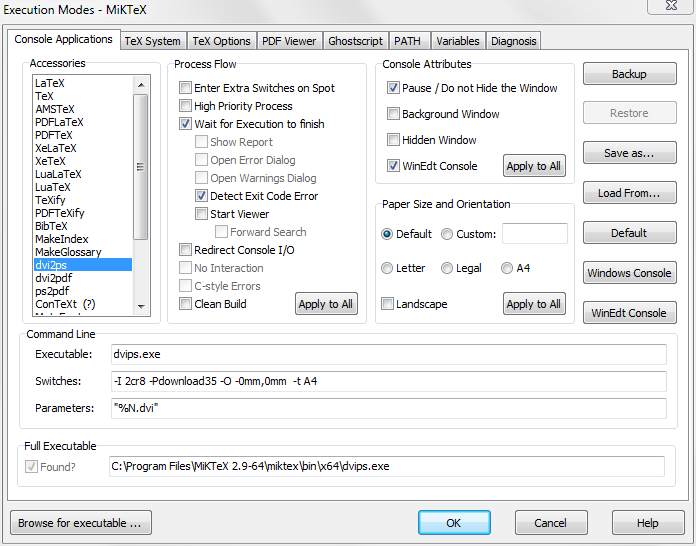
\includegraphics[bb=0 0 696 546,width=\textwidth]{eps/dvipsbmeps.png}}

\subsection{Enable JPG Images in DVIPS}

bm2eps also converts jpeg files, just use it as follows:

{\small
\verb"\centerline{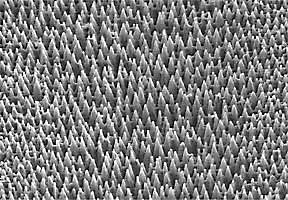
\includegraphics[bb= 0 0 288 200,width=0.5\textwidth ]{pic/light_trap2.jpg}}"
}


\centerline{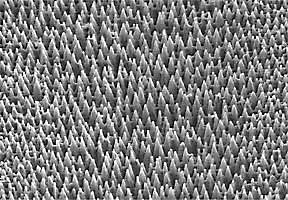
\includegraphics[bb= 0 0  288 200,width=0.5\textwidth]{pic/light_trap2.jpg}}




\subsection{Control Font Download to the PS File}

In the previous graph the dvi2ps application is also instructed to download the `standard Adobe' fonts to the PS file, by entering the option

\lstinline{ -Pdownload35}


\subsection{Setting up the Page Size for dvi2ps}

To set the page size in dvi2ps, add the following additional text to the dvi2ps switches:

\lstinline{-I 2cr8 -Pdownload35 -O -0mm,0mm  -t A4}


\subsection{Setting up the Page Size for ps2pdf}

Activate
$<$Options$>$$<$Execution Modes$>$ and select the ps2pdf entry in the 'Accessories' list box. Then change the page size as shown in the next figure. It does not make sense that the A4 should be in effect when the page size is set to default, but it does seem to work.

\centerline{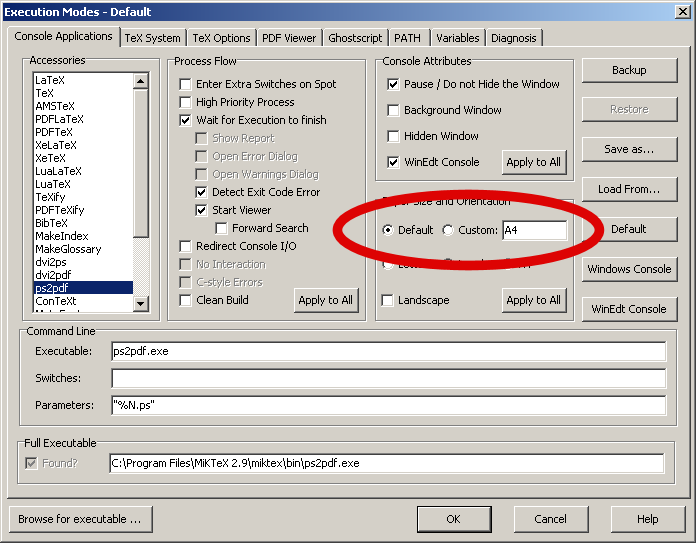
\includegraphics[bb= 0 0 696 543,width=\textwidth]{eps/ps2pdfpagesize.png}}

%Open the file \verb"C:\Program Files\WinEdt Team\WinEdt 10Exec\TeX\ps2pdf.edt"
%and do the following change
%
%\begin{verbatim}
%  //LetReg(4,'');
%  LetReg(4, "%!4 -sPAPERSIZE=a4");
%\end{verbatim}






\section{PostScript Specials and Security}

The issue discussed here became evident in Miktex 2.5, but could also apply to any other application that uses DVIPS.  The problem presented itself as an inability of YAP to preview some DVI pages.


As from Version 5.95b DVIPS does not support 'unsecure' path names, such as \\
- absolute path names (like C:/temp/eurotour.eps)\\
- parent-relative path names (like ../../temp/eurotour.eps)\\
which means that the following will not work:\\
\verb+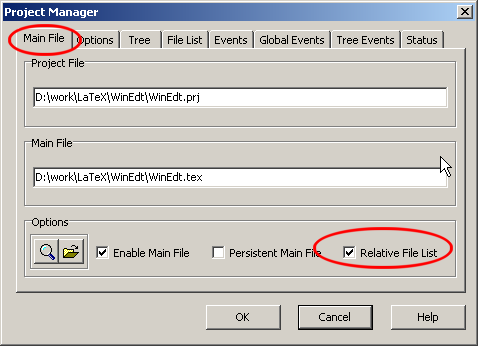
\includegraphics[bb= 0 0 512 387,scale=0.7]{eps/projectmanager.png}+

YAP complains with a message similar to:
{\small
\begin{verbatim}
MiKTeX Problem Report
Message: The page could not be rendered.
Data: This is dvips(k) 5.95b Copyright 2005 Radical Eye Software (www.radicaleye.com)
' TeX output 2006.05.28:2135' ->
<tex.pro><texps.pro><special.pro>. <cmbx12.pfb><cmr10.pfb>[2<eurotour.eps>
C:\Program Files\MiKTeX 2.5\miktex\bin\dvips.exe:
Could not find figure file c:/temp/eurotour.eps; continuing
\end{verbatim}
}

On Cristian Schenk's page he states:\\
(\verb+http://dojo.miktex.org/blogs/christian_schenk/archive/2006/03/06/328.aspx+)

{\small
\begin{verbatim}
It would be possible to break these security rules by
- using the Dvips option -R0
- by specifying z0 in the Dvips configuration file
\end{verbatim}
}

Schenk offered to implement the first option with a future release of YAP, but as of version 2.7 is still is not implemented.  Our recourse is then to implement the second option ourselves.

On my PC,the DVIPS config file, \verb"config.ps", is located at the following location:

\verb+C:\Program Files\MiKTeX 2.7\dvips\config+

In this file, find these lines:

\begin{verbatim}
% z1 is "secure", i.e., inhibits execution of `shell commands` in
% \specials.  Dvips allows this by default.
z1
\end{verbatim}

and change it to this:

\begin{verbatim}
% z1 is "secure", i.e., inhibits execution of `shell commands` in
% \specials.  Dvips allows this by default.
z0
\end{verbatim}

At the top of the config file it instructs us to use \verb"initexmf" to change this file, but I could not find an easy way to do this, so I just manually edited \verb"config.ps".  It seems to work.



